\documentclass[10pt,a4paper]{report}
\usepackage[utf8]{inputenc}
\usepackage[spanish]{babel}
\usepackage{amsmath}
\usepackage{graphicx}
\usepackage{braket}
\usepackage{amsfonts}
\usepackage{amssymb}
\author{Pablo Enrique Yanes Thomas}
\title{Candidatura}
\makeindex

\begin{document}

\tableofcontents
\chapter*{Objetivo General}

Se busca modelar un sistema optomecánico con parámetros dependientes del tiempo. El sistema es una cavidad de Fabry-Perot donde uno de los dos espejos es un resonador armónico cuya frecuencia natural depende del tiempo de manera periódica. Se ha demostradon que utilizar un formalismo que toma en cuenta la dependencia temporal de la frecuencia natural del oscilador llevan a un mejor modelo teórico para el sistema\cite{HanngiFM}. En un trabajo anterior donde se utiliza este formalismo para estudiar el enfriamiento del oscilador mecánico se encontró que la predicción para el enfriamiento es cualitativamente distinta aún a primer orden de perturbación para la dependencia temporal\cite{YanesOC}. Esto motiva la pregunta: ¿Qué sucede al tomar en cuenta el efecto de la variación de la longitud de la cavidad sobre la frecuencia de resonancia de la cavidad? En este trabajo se investiga este efecto. 


\chapter{Introducción}

La optomecánica es el estudio de la interacción entre elementos ópticos y elementos mecánicos. En este capítulo se dará una breve introducción al tipo de sistemas y de efectos que se consideran parte de la optomecánica. 


\section{Posibles Sistemas Optomecánicos}

Existen muchas implementaciones posibles de acoplamientos entre elementos ópticos y elementos mecánicos \cite{KippenberCO}. En esta sección se detallan algunas de las posibilidades.

\subsection{Espejos Suspendidos}

Estos sistemas consisten en cavidades ópticas donde uno o más de los espejos pueden cambiar de posición y así alteran la longitud de la cavidad. La primera realización experimental de este tipo de sistemas se debe a los primeros esfuerzos para detectar ondas gravitacionales \cite{AbramoviciLIGO}. El sistema consiste en un interferómetro con los espejos fijos en masas suspendidas, a manera que una onda gravitacional, al interactuar con las masas cambiaría la posición de los espejos y así la longitud de camino óptico. El propósito de suspender las masas no es optomecánico, sin embargo, las fluctuaciones en la potencia del láser, debido a la incertidumbre en el número de fotones, son un efecto cuántico que impone un límite a la precisión de las mediciones \cite{CavesIF}. Experimentos en este tipo de sistemas han demostrado varios efectos, entre ellos el enfriamiento mediante presión de radiación \cite{CorbittOC}. También es posible utilizar este tipo de sistemas para estudiar el entrelazamiento cuántico\cite{ChenED} al acoplar dos cavidades al mismo espejo y así lograr entrelazamiento entre los modos de ambos campos.

\subsection{Microresonadores}

Otro tipo posible de sistema son los microresonador o microcavidades. En este tipo de sistemas, es posible confinar a la luz a viajar en modos \textit{whispering gallery}, los cuales implican que la luz es guiada a lo largo del perímetro del resonador,el cual puede tener forma esférica, circular, o toroidal\cite{VahalaOM}. Si este vibra, esto puede alterar el camino óptico de la luz y se logra un acoplamiento optomecánico. Es posible fabricar resonadores de este tipo con un factor de calidad de $10^6$ \cite{EuroSensors2017}. Debido a su tamaño, es posible obtener acoplamiento fuerte entre sistemas cuánticos y el resonador\cite{VerhagenMOC}.

\subsection{Objetos Suspendidos o Levitados}

En este tipo de sistemas, se considera una cavidad óptica rígida donde se coloca un objeto mecánico dentro de la cavidad. Este esquema permite el acoplamiento de objetos mecánicos de tamaños inferiores a la longitud de onda de la luz \cite{KippenberCO}, como por ejemplo una membrana dieléctrica de $SI_3N_4$ de  $1mm \times 1mm \times 50nm$
de dimensión\cite{SankeyMC}. En ese caso, se puede observar que parámetros de la cavidad como la sintonización y la finesa dependen del desplazamiento de la membrana. Otra posibilidad consiste en un nano cable de carbón, de aproximadamente $10^9$ átomos, el cual se coloca dentro de una micro cavidad de Fabri-Perot. Así mismo, se han realizado experimentos donde se levita una gota de Helio líquido dentro de la cavidad\cite{ChildressLD}. Las propiedades de la cavidad cambian no solo dependiendo de la posición del objeto, sino también de sus modos vibracionales\cite{FaveroCR}.  

\subsection{Cristales Optomecánicos}

Este tipo de sistema es más reciente que los demás y se basa en redes cristalinas donde se logra acoplar fotones y fonones. En primera instancia se fabricó una nano viga de silicio  \cite{EichenfieldOC}. El sistema consiste en una nano viga con agujeros espaciados regularmente, lo cual forma una red. Se introduce un defecto mediante una reducción cuadrática en la constante de red, de manera simétrica al centro de la viga. Esto genera un potencial efectivo para los modos ópticos y uno análogo para los modos mecánicos. Las vibraciones ocasionan un cierto desplazamiento en la estructura lo cual afecta el potencial efectivo para los modos ópticos y se obtiene el acoplamiento. Una implementación reciente de este tipo de sistemas involucra usar redes cristalinas semi periódicas de diamante para implementar el resonador\cite{BurekDO}.

\section{Efectos Optomecánicos}

En esta sección se da un pequeño resumen de los efectos optomecánicos más conocidos y utilizados. Frecuentemente estos efectos de deben a la interacción entre la presión de radiación que la luz incidente aplica sobre los elemento mecánicos y la reacción retardada de la cavidad a los cambios en su estructura. Algunos de estos efectos son:


\begin{itemize}
\item \textbf{Efecto de Resorte Óptico (optical spring effect)} La presión de radiación depende la posición del objeto, por lo que esta cambia cuando el objeto se mueve. En particular, en el caso de cavidades con espejos suspendidos, la presión de radiación afecta la constante del resorte ya que genera un desplazamiento en la resonancia de la frecuencia mecánica, el cual se puede utilizar para aumentar o disminuir la frecuencia natural del resorte.\cite{BraginskyPE}

\item \textbf{Bi-Estabilidad Óptica (optical bi-stability)} La presión de radiación puede desplazar al objeto mecánico y se espera que se llegue a una posición de equilibrio. Sin embargo, la dependencia del potencial efectivo sobre la posición es no lineal, lo cual lleva a que se generen dos posiciones de equilibrio. Para una presión lo suficientemente fuerte, este efecto se borra y se llega a una posición altamente estable\cite{DorselOB}.

\item \textbf{Enfriamiento Optomecánico}  A la absorción de fonones (enfriamiento) se le asocia con procesos de dispersión de Raman donde un quanto sube de nivel mientras que los procesos de emisión (calentamiento) se le asocia con dispersión de Raman donde un fotón decae \cite{LCNooshi}. Este enfriamiento es posible siempre y cuando el ancho de banda de la cavidad sea mucho menor que la frecuencia de oscilación mecánica. \cite{LCNooshi} \cite{MarquardtSC} Este régimen solo es válido cuando el acoplamiento optomecánico puede ser tratado como una perturbación, así que el esquema deja de ser valido cuando el acoplamiento es comparable al ancho de banda de la cavidad o a la frecuencia del oscilador mecánico
\end{itemize}


\section{Aplicaciones}

Existen muchas aplicaciones posibles para los efectos y sistemas utilizados en optomecánica. Este trabajo se concentra principalmente en enfriamiento optomecánico, sin embargo algunas otras posibles aplicaciones son:

\begin{itemize}

\item \textbf{Estabilización Laser} Al utilizar una cavidad de tipo cristal optomecánico doble (\textit{zipper cavity} en inglés) como base para un láser, se puede obtener un dispositivo tal que su frecuencia, en especial la sensibilidad de está a ruido térmico, se puede estabilizar optomecanicamente\cite{MayerZC}.

\item  \textbf{Memoria Optomecánica} Se puede crear un sistema de memoria utilizando una cavidad optomecánica compuesta por una guía de ondas y un resonador mecánico ligeramente torcido a manera de tener dos configuraciones posibles, arriba y abajo. Esto lleva a que se genere un potencial de doble pozo asimétrico para el resonador y con la ayuda de un láser para excitar el sistema y de otro para enfriarlo es posible realizar un proceso controlado donde se decide en que pozo queda el resonador. Estos dos estados corresponden a 0 y 1 y el sistema no requiere energía para mantenerse en la configuración final, generando un sistema de memoria estable \cite{BagheriMM}.

\item \textbf{Magnetometría} Al acoplar un material magnetostrictivo al resonador mecánico de una cavidad optomecánica se pueden excitar los eigenmodos del resonador mecánico al aplicar un campo magnético. De esta forma, la presencia del campo magnético se puede leer en el comportamiento del campo de luz dentro de la cavidad. Esto permite tener un sensor de campos magnéticos de alta precisión que funciona a temperatura ambiente \cite{ForstnerOM}.

\item \textbf{Reder Cuánticas} La optomecánica permite realizar el mapeo de los estados de un campo de luz a los modos vibracionales de un oscilador mecánico \cite{ZhangQST}. Este tipo de transferencia de información es clave en la formación de redes de información cuánticas.\cite{KimbleQI}

\item \textbf{Detección de Cáncer} Los Microtúbulos son una parte clave de la estructura de una célula y se ha estudiado si su interacción con campos electromagnéticos externos puede ser un tratamiento viable para el cáncer\cite{KirsonEMT}. El estudio de las propiedades vibracionales de estas estructuras es clave para esto y se ha propuesto un montaje experimental para realizar estas mediciones mediante un acoplamiento optomecánico\cite{SalariOC}.

\end{itemize} 

\section{Enfriamiento Optomecánico con Parámetros Dependientes del Tiempo}

Este trabajo se enfoca en el enfriamiento optomecánico con parámetros dependientes del tiempo. Uno de los métodos empleados la búsqueda por mejorar el enfriamiento del oscilador mecánico acoplado a la cavidad es utilizar un oscilador mecánico cuya frecuencia natural sea función del tiempo \cite{BarberisLC}. Esta dependencia modifica el cuasi espectro de energía del sistema\cite{HanngiFM}. En el acercamiento empleado en \cite{BarberisLC} esto no se toma en cuenta, sin embargo, dado que \cite{HanngiFM} muestra que este no es el enfoque óptimo, se realizó un trabajo que sí toma en cuenta los efectos de la dependencia temporal de la frecuencia natural del oscilador durante la derivación  de la temperatura final que se espera del sistema \cite{YanesOC}. Los resultados de este trabajo muestras diferencias cuantitativas y cualitativas en el comportamiento de la temperatura del oscilador mecánico, lo cual motiva la pregunta ¿qué sucede al tomar en cuenta la dependencia temporal de la frecuencia del oscilador mecánico sobre la frecuencia natural de la cavidad? 

En esta propuesta se explican los pasos que se siguen para modelar este tipo de sistemas en términos generales y luego se explica como se obtiene la temperatura final del sistema. Finalmente se propone aplicar este formalismo a un sistema donde se toma en cuenta la dependencia temporal de tanto un oscilador mecánico como la cavidad a la cual este se encuentra acoplado. Se discute la teoría de los sistemas cuánticos abiertos, del oscilador mecánico dependiente del tiempo, y el enfriamiento optomecánico dependiente del tiempo.




\chapter{Oscilador Armónico Dependiente del Tiempo}

Antes de proceder a enfriamiento optomecánico es importante saber como modelar de manera cuántica un oscilador armónico con frecuencia dependiente del tiempo. Para resolver el problema, se utiliza la teoría de Floquet \cite{WardFT} y se busca una expresión para el Hamiltoniano del sistema expresada en términos de operadores de Floquet, los cuales se definirán más adelante.

\section{Teoría de Floquet}

Se desea resolver una ecuación diferencial que involucra coeficientes con dependencia temporal, tal como

\begin{equation}\label{FloquetEquation}
x' = A(t)x,
\end{equation} donde la función $A(t)$ es periódica con periodicidad $\tau$. En este caso el teorema de Floquet\cite{WardFT} dice que la solución no necesariamente es periódica pero debe tener la forma

\begin{equation}\label{FloquetForm}
x(t)=e^{\mu t}p(t).
\end{equation} Los valores $\mu$ se conocen como los exponentes característicos o de Floquet y la función $p(t)$ es periódica con período $\tau$, es decir el mismo periodo que el coeficiente en la ecuación diferencial. Los coeficientes $\mu$ son, en general, complejos. Claramente, el hecho de que la solución tenga la forma \eqref{FloquetForm} puede llevar a que la solución se dispare con el tiempo, por lo que se desea entender el criterio de estabilidad de este tipo de soluciones. Antes de esto, es necesario establecer algunas definiciones y propiedades, las cuales se presentan sin demostración debido a que no son el enfoque principal de este trabajo. Si el lector se encuentra interesado, el tratamiento se encuentra con mayor detalle en las notas de las cuales surge la sección siguiente \cite{WardFT}.

\subsection{Propiedades Básicas}

Sea la ecuación \eqref{FloquetEquation} en $n$ dimensiones. Esto es, se piensa en $x$ como un vector de $n$ dimensiones y en $A(t)$ como una matriz de $n \times n$. En este caso, si la ecuación tiene $n$ soluciones $x_1, x_2, ... , x_n$, se define la \textbf{matriz fundamental} como la matriz formada utilizando las soluciones como columnas, siempre y cuando estas sean linealmente independientes

\begin{equation}
X(t) = [[x_1][x_2]...[x_n]],
\end{equation}Si $X(t_0) = I$ la matriz se conoce como la \textbf{matriz fundamental principal}. Se tiene que

\begin{center}
\textbf{Lema:} \textit{Si $X(t)$ es una matriz fundamental, también lo es $X(t)C$ para cualquier matriz constante y no singular $C$.}
\end{center}Y que

\begin{center}
\textbf{Lema:} \textit{Sea $W(t)$ el Wronskiano de $X(t)$ el determinante de X(t), entonces:}

\begin{equation}
W(t) = W(t_0) e^{\int_{t_0}^{t}tr[A(s)]ds}.
\end{equation}
 
\end{center} Se tiene entonces un teorema

\begin{center}
\textbf{Teorema:} \textit{Sea A(t) una matriz con periodicidad $\tau$. Si $X(t)$ es una matriz fundamental entonces $X(t+\tau)$ también lo es y existe una única matriz constante no singular $B$ tal que:}\linebreak \linebreak i) $X(t+\tau) = X(t)B \qquad\forall t$, \linebreak ii) $det(B) = e^{\int_0^t tr[A(s)]ds}.$
\end{center}Si se toma $X(0)=I$ entonces $B=X(\tau)$. Con esto se pueden definir los \textbf{multiplicadores característicos}, los cuales son los valores propios de la matriz $B$, y se denominan con la letra $\rho$. Estos cumplen que

\begin{equation}
\rho_1 = e^{\mu_1 \tau}, \quad \rho_2 = e^{\mu_2 \tau}, ... , \rho_n = e^{\mu_n \tau},
\end{equation} donde los valores $\mu$ son los exponentes de Floquet definidos anteriormente. Se cumplen cuatro propiedades:

1) Los multiplicadores característicos de $B=X(\tau)$ cumplen que

\begin{equation}
det(B) = \rho_1 \rho_2 ... \rho_n = e^{\int_0^T tr[A(s)]ds}.
\end{equation}

2) Trivialmente, como la traza es la suma de los valores propios

\begin{equation}
Tr[B] = \rho_1 + \rho_2 + ... + \rho_n.
\end{equation}

3) Los multiplicadores característicos no son únicos, ya que

\begin{equation}
e^{\mu \tau} = e^{(\mu  +\frac{2\pi i}{\tau} )\tau}.
\end{equation}

4) Los multiplicadores característicos son una propiedad de la ecuación \eqref{FloquetEquation} y no dependen de la elección de matriz fundamental.

Con estas propiedades, se puede pasar a analizar la estabilidad de las soluciones para el caso específico de ecuaciones de segundo orden.

\subsection{Estabilidad para Ecuaciones de Segundo Orden}\label{EstabilidadSO}

Si se piensa en una ecuación diferencial de segundo orden del tipo

\begin{equation}
\ddot{x} + a(t)x= 0,
\end{equation} donde $a(t)$ tiene periodo $\tau$. Si se toma $x_1 = x$ y $x_2 = \dot{x}$, la ecuación puede re-escribirse como

\begin{equation}
[\begin{array}{c}
\dot{x_1} \\
\dot{x_2}
\end{array}] = [\begin{array}{cc}
0 & 1 \\
-a(t) & 0
\end{array}][\begin{array}{c} 
x_1 \\ 
x_2

\end{array}],
\end{equation} si se toma la condición inicial $[\begin{array}{c} 1 \\ 0 \end{array}]$, se obtiene una solución de la forma

\begin{equation}
[\begin{array}{c}
x_1^1(t) \\
\dot{x_1^1(t)}
\end{array}],
\end{equation} y para la condición inicial $[\begin{array}{c} 0 \\ 1 \end{array}]$, se obtiene una solución de la forma

\begin{equation}
[\begin{array}{c}
x_1^2(t) \\
\dot{x_1^2(t)}
\end{array}],
\end{equation} esto permite generar la matriz $B$

\begin{equation}
B= [\begin{array}{cc}

x_1^1(\tau) & x_1^2(\tau) \\
\dot{x_1^1(\tau)} & \dot{x_1^2(\tau)}

\end{array}],
\end{equation} lo cual permite calcular los multiplicadores característicos, ya que

\begin{equation}
\rho_1 \rho_2 = e^{\int_0^\tau Tr[A(s)]ds} = e^0 = 1,
\end{equation} y

\begin{equation}
\rho_1 + \rho_2 = Tr[B] =x_1^1(\tau)+ \dot{x_1^{(2)}(\tau)} = 2\phi.
\end{equation} Esto permite obtener la ecuación

\begin{equation}
\rho = \phi \pm \sqrt{\phi^2 -1},
\end{equation} o en términos de $\mu$

\begin{equation}
cosh(\mu_1 \tau) = \phi.
\end{equation} Esto lleva a analizar cinco situaciones distintas.

\textbf{Caso $ -1 < \phi < 1$}: En este caso, para algún valor $\sigma$ se tiene que $\phi = cos(\sigma \tau)$ por lo que:

\begin{align*}
\rho =& \phi \pm \sqrt{\phi^2 -1},\\
=& cos(\sigma \tau) \pm isen(\sigma \tau), \\
=& e^{\pm i\sigma \tau},
\end{align*} lo cual lleva a una solución general de tipo:

\begin{equation}
x(t) = c_1 Re(e^{i\sigma t} p(t)) + c_2 Im(e^{i\sigma t} p(t)),
\end{equation} la cual es estable y pseudo periódica.

\textbf{Caso $1 < \phi$:} en este caso $\rho > 1$ y como $\rho_1 = \frac{1}{\rho_2}$, tenemos que $\mu_1 = -\mu_2$. Por esto, la solución es de la forma:

\begin{equation}
x(t) = c_1 e^{\mu_1 t}p_1(t) + c_2 e^{\mu_2 t}p_2(t)
\end{equation} donde las funciones $p(t)$ son periódicas con periodo $\pi$. La solución es inestable.

\textbf{Caso $\phi < -1$:} en este caso se tiene una solución del tipo:

\begin{equation}
x(t) =c_1 e^{\gamma_1 t}q_1(t) + c_2 e^{-\gamma_2 t}q_2(t),
\end{equation} donde las funciones $q(t)$ tienen periodo $2\pi$ y los coeficientes $\gamma = \mu + \frac{i\pi}{\tau}$. La solución de nuevo es inestable.

\textbf{Caso $\phi = -1$:} para este caso también se tiene una solución inestable, de la forma:

\begin{equation}
x(t) = (c_1 + tc_2)q_1(t) + c_2q_2(t)
\end{equation} de nuevo la funciones $q(t)$ tienen periodo $2\pi$.

\textbf{Caso $\phi = 1$:}

para este caso también se tiene una solución inestable, de la forma:

\begin{equation}
x(t) = (c_1 + tc_2)p_1(t) + c_2p_2(t)
\end{equation} de nuevo la funciones $p(t)$ tienen periodo $\pi$.

Es muy importante notar que en estos dos últimos casos, esta forma de la solución solo es correcta si la matriz $B$ tiene un solo eigenvector linealmente independiente. Si este no es el caso, la solución tiene la forma usual con las funciones $p(t)$ o $q(t)$, estos dos casos marcan el límite entre la estabilidad y la inestabilidad en este problema. Finalmente, se verá como estos criterios aplican a una ecuación que será relevante más adelante, la ecuación de Hill.

\subsection{Estabilidad de las Soluciones de Floquet para la Ecuación de Hill}

La ecuación de Hill es una ecuación diferencial de segundo orden con coeficientes dependientes del tiempo de forma periódica\cite{WardFT}

\begin{equation}
\ddot{x}(t) + (\delta + \epsilon b(t))x = 0,
\end{equation} nuevamente, la función $b(t)$ tiene periodo $\tau$ y se considera que $\delta$ y $\epsilon$ son constantes reales. Para el caso $\epsilon = 0$ claramente la ecuación se reduce al oscilador armónico usual y las soluciones son estables. Sin embargo, para ciertos valores de $\delta$ puede encontrarse la región donde la solución aún es periódica, esto se puede resolver para los casos $\phi = \pm 1$, donde $\phi$ es la función definida en la sección \eqref{EstabilidadSO}, de forma que se tiene soluciones estables y periódicas para los casos

\begin{equation}
\delta = (2m\frac{\pi}{\tau})^2, 
\end{equation} que corresponde a $\phi=1$ y

\begin{equation}
\delta = ((2m+1)\frac{\pi}{\tau})^2,
\end{equation} que corresponde a $\phi=-1$. Estos valores representan la frontera de la región de soluciones estables, las cuales corresponden a periodo de $\tau$ y $2\tau$ respectivamente. Más adelante se buscaran soluciones en esta región para el caso donde $\epsilon \ll 1$.


\section{Estados de Floquet en Mecánica Cuántica}

Ahora se busca estudiar Hamiltonianos con una dependencia periódica en el tiempo, donde se utilizaran los resultados obtenidos en la sección anterior

\begin{equation}
H(t)=H(t+\tau).
\end{equation} El hecho de que el Hamiltoniano sea simétrico respecto a (ciertas) traslaciones en el tiempo, permite el uso del formalismo de Floquet \cite{HanngiDQS}. Se asume que la dependencia temporal puede ser vista como una perturbación sobre un Hamiltoniano original

\begin{equation}
H(x,t)=H_0(x)+V(x,t) \qquad V(x,t)=V(x,t+\tau).
\end{equation} Se utiliza que el Hamiltoniano no perturbado posee un conjunto completo de eigenfuciones $\{\phi_n\}$ con valores propios correspondientes $E_n$. En este caso, la ecuación de Schr\"{o}dinger tiene la forma

\begin{equation}\label{SchrodingerEQ}
-i\hbar\dot{\Psi}(x,t) = H(x,t)\Psi(x,t).
\end{equation} El problema cumple con las condiciones necesarias para utilizar una solución del tipo visto en la sección anterior

\begin{equation}
\Psi_n(x,t) = e^{(\frac{-i}{\hbar}\mu_nt)}\Phi_n(x,t).
\end{equation} Como se mencionó en la sección anterior, $\mu$ en general es un número complejo, lo cual puede llevar a soluciones inestables. En este caso $\Phi_n(x,t)$ es la función que contiene la periodicidad en el tiempo. Sustituir la solución en la ecuación \eqref{SchrodingerEQ} genera una ecuación para las funciones periódicas

\begin{equation}
H(x,t)\Phi_n(x,t)=E_n\Phi_n(x,t).
\end{equation} Antes de buscar formas explícitas para estos estados, es necesario resolver el problema clásico correspondiente a este sistema. La razón para esto se verá más adelante, y se debe sencillamente a que estas soluciones clásicas juegan un papel clave en las expresiones explícitas para los estados y operadores involucrados en la solución del problema cuántico.

\section{Oscilador Armónico Dependiente del Tiempo: Solución Mediante Formalismo de Floquet}

En el caso clásico \cite{HanngiFM} se tiene, para un oscilador armónico unidimensional con frecuencia dependiente del tiempo y el cual experimenta una fuerza disipadora dependiente de la velocidad, que la posición cumple

\begin{equation}
\ddot{x}+\gamma\dot{x}+\frac{k(t)}{m}x=0
\end{equation}

Se asume que la función $k(t)$ es periódica con periodo $T$. Si se utiliza la sustitución $x=ye^{-\frac{\gamma t}{2}}$, se llega a la ecuación

\begin{equation}
\ddot{y} +(\frac{k(t)}{m}-\frac{\gamma^2}{4})y=0
\end{equation}

El teorema de Floquet para ecuaciones de segundo orden con coeficientes del tiempo \cite{HanngiFM} asegura que esta ecuación tiene dos soluciones

\begin{equation}
E_1(t) = e^{i\mu t}\phi(t), \quad E_2(t)=E_1(-t),
\end{equation} Recordando que la función $\phi$ debe tener la misma periodicidad que $k(t)$. Dado que la función cumple con esta condición, es posible realizar una expansión de Fourier \cite{ArfkenMM} de la misma

\begin{equation}
\phi(t) = \sum_{-\infty}^\infty c_n e^{in\omega t}.
\end{equation} Para fijar los coeficientes se elije una normalización tal que el Wronskiano sea

\begin{equation}
W = \dot{E}_1(t)E_2(t)-E_1(t)\dot{E}_2(t) = 2i.
\end{equation}Esto genera la regla de suma

\begin{equation}
\sum_{-\infty}^\infty c_n^2(\mu + n\omega) = 1,
\end{equation} y permite, en teoría, calcular las constantes de la expansión para un caso general. A continuación se trata el caso en mecánica cuántica.

\section{Caso Cuántico}

En el caso de un Hamiltoniano con dependencia temporal como la vista anteriormente, existe un conjunto completo de soluciones \cite{BarnettSD}

\begin{equation}
\Ket{\Psi_\alpha (t)} = e^{-i\mu_\alpha t}\Ket{\phi_\alpha t}, \qquad \Ket{\phi_\alpha (t)}=\Ket{\phi_\alpha (t+\tau)},
\end{equation}

Estas soluciones tienen la forma explícita\cite{BrownPT}

\begin{equation}
\Psi_\alpha (x,t) = (\frac{\sqrt{m/\pi\hbar}}{2^\alpha n!E_1^0(t)})^{\frac{1}{2}}(\frac{E_1^0(t)}{E_2^0(t)})^\frac{\alpha}{2}H_\alpha(x\sqrt{\frac{m}{\hbar E_1^0(t) E_2^0(t)}})e^{(ix^2\frac{E_1^0(t)}{2E_2^0(t)})}
\end{equation} donde el superíndice cero indica que se toma el límite donde $\gamma$ tiende a cero. Sin embargo, estas soluciones se comportan de manera análoga a los estados de la base de Fock bajo la acción de los operadores de Floquet, los cuales pueden expresarse en términos de los operadores de momento y posición usuales en mecánica cuántica

\begin{equation}\label{FloquetOperators}
\Gamma(t) = \frac{1}{2i}(\hat{x}\dot{E}_1^0(t)\sqrt{\frac{2}{\hbar m}}-\hat{p}E_1^0(t)\sqrt{\frac{\hbar}{2m}}).
\end{equation} Así como su complejo conjugado. Su acción sobre la base de Floquet queda definida por

\begin{align*}
\Gamma(t) \Ket{\Psi_\alpha (x,t)} =& \sqrt{\alpha}\Ket{\Psi_{\alpha-1} (x,t)}, \\
\Gamma^\dagger(t) \Ket{\Psi_\alpha (x,t)} =& \sqrt{\alpha+1}\Ket{\Psi_{\alpha+1} (x,t)}.
\end{align*}Es importante notar que estos operadores dependen explícitamente del tiempo. Es conveniente entender el origen de estos operadores. Se toma entonces un Hamiltoniano usual de oscilador armónico, con la excepción de que la frecuencia del oscilador es una función periódica del tiempo

\begin{equation}\label{TDHO}
H = \frac{1}{2m}p^2 + \frac{1}{2}k(t)q^2.
\end{equation} Este lleva a la ecuación de movimiento usual

\begin{equation}
m\ddot{q}(t) + k(t)q(t) = 0,
\end{equation} para el operador $q(t)$. Lo que se busca es una transformación unitaria que lleve este problema al problema usual del oscilador armónico en mecánica cuántica. Se trabaja en el cuadro de Heisenberg \cite{SakuraiQM}, tal que

\begin{align}
\tilde{q}(t) =& U^{-1}(t)q(t)U(t),\\
\tilde{p}(t) =& U^{-1}(t)p(t)U(t).
\end{align} Y donde entonces el nuevo Hamiltoniano queda dado por

\begin{equation}
\tilde{H} = H + U^{-1}i\dot{U}.
\end{equation} Para la transformación se elige

\begin{equation}
U = e^{-i\chi(t)q^2(t)},
\end{equation} donde

\begin{equation}
\chi(t) = \frac{m}{4}(\frac{\dot{f}}{f}+\frac{\dot{f^*}}{f^*})
\end{equation} Las funciones $f$ son las soluciones al problema clásico correspondiente al Hamiltoniano \eqref{TDHO} el cual tiene dos soluciones linealmente independientes, pero una es la compleja conjugada de la otra. Estas soluciones corresponden a $E_1^0$  y $E_2^0$ vistas en la sección anterior. Bajo esta transformación

\begin{align}
\tilde{q}(t)=&q(t),\\
\tilde{p}(t)=&p(t)-2\chi(t)q(t).
\end{align}Utilizando esto se puede escribir el Hamiltoniano en las nuevas coordenadas tomando en cuenta que $\ddot{f}= -k(t)f$ y el Wronskiano, $W$

\begin{equation}
 H = \frac{1}{2m}\tilde{p}^2 + \frac{\chi(t)}{m}(\{\tilde{q},\tilde{p}\}) + \frac{mW^2}{|f|^2}k(t)\tilde{q}^2.
\end{equation}Para eliminar el término cruzado se utiliza una segunda transformación

\begin{equation}
U_2(t)=e^{\frac{i}{4}(\{\tilde{q},\tilde{p}\})ln|f|^2}.
\end{equation}Esto es una transformación de escala que deja como variables finales

\begin{align}
Q=&U_2^{-1}\tilde{q}U_2 =\frac{1}{|f|}q(t),\\
P=&U_2^{-1}\tilde{p}U_2 = |f|(p-2\chi q), 
\end{align} en estas variables, el Hamiltoniano es

\begin{equation}\label{QTDHO}
\tilde{H} = \frac{1}{|f(t)|^2}(\frac{1}{2m}P^2(t)+\frac{1}{2}mW^2Q^2(t)).
\end{equation}Este Hamiltoniano es, salvo por un coeficiente general dependiente del tiempo, el Hamiltoniano usual de oscilador armónico y se puede resolver por medio de operadores de escalera

\begin{equation}
\Gamma = \sqrt{\frac{mW}{2}}Q + i \sqrt{\frac{1}{2mW}}P.
\end{equation} La expresión \eqref{FloquetOperators} se obtiene expresando los operadores en las coordenadas usuales, no en las transformadas. Es de mas utilidad expresar este Hamiltoniano en terminos de estos operadores $\Gamma(t)$. Se obtiene

\begin{equation}
\tilde{H} = \frac{W}{|f(t)|^2}(\Gamma^\dagger(t)\Gamma(t) + \frac{1}{2}).
\end{equation}

Con esto establecido se puede proceder a establecer un Hamiltoniano para enfriamiento optomecánico con parámetros dependientes del tiempo.

\chapter{Enfriamiento Optomecánico Dependiente del Tiempo}

\section{Hamiltoniano para Enfriamiento Optomecánico con Parámetros Dependientes del Tiempo}

En particular, se analiza un sistema tal que la frecuencia natural del oscilador mecánico depende del tiempo de manera periódica. Se asume que el oscilador se encuentra acoplado a un único modo forzado de la cavidad el cual tiene frecuencia $\omega_{cav}$. Se asume que el marco de referencia rota con la frecuencia de la bomba. Se modela el sistema mediante el siguiente Hamiltoniano\cite{BarberisLC}

\begin{equation}
H(t) = H_{cav} + H_{mec}(t) + H_{rad} + H_{Bomba}.
\end{equation} En donde

\begin{align}
H_{cav} =& -\hbar \delta a^\dagger a,\\
H_{mec}(t) =& \frac{p^2}{2m} + \frac{1}{2}m \nu^2 (t) x^2,\\
H_{rad} =& -\hbar g a^\dagger a x,\\
Bomba =& \hbar\frac{\Omega}{2}(a^\dagger + a),
\end{align} en este caso, $\delta = w_{bomba} - w_{cav}$ representa la diferencia de frecuencias entre la bomba de fotones y la cavidad y $\hbar g$ representa la fuerza de radiación que un fotón aplica sobre el oscilador mecánico sin modulación. El término $H_{rad}$ modela una interacción simple entre los fotones y el espejo. Dado que en este caso la longitud de la cavidad no es fija, la frecuencia de la cavidad debe tener una dependencia en la coordenada $x$, entonces, tomando el Hamiltoniano para el oscilador que modela la cavidad y expandiendo hasta primer orden en $x$ (el resultado obtenido mediante un procedimiento más completo es el mismo)\cite{KippenberCO} 

\begin{equation}
\hbar w_{cav}(x) a^\dagger a \simeq \hbar(w_{cav}-g_0x)a^\dagger a,
\end{equation}lo cual acopla los dos sistemas. Por \eqref{QTDHO}, se modela al oscilador mecánico utilizando operadores de Floquet

\begin{equation}
H_{mec}(t) = \hbar\frac{W}{|f(t)|^2}(\Gamma^\dagger \Gamma + \frac{1}{2}).
\end{equation} Recordando la definición de los operadores de Floquet \eqref{FloquetOperators}, se puede invertir la relación en términos de los operadores $x$ y $p$

\begin{align*}
\Gamma(t) \Ket{\Psi_\alpha (x,t)} =& \sqrt{\alpha}\Ket{\Psi_{\alpha-1} (x,t)}, \\
\Gamma^\dagger(t) \Ket{\Psi_\alpha (x,t)} =& \sqrt{\alpha+1}\Ket{\Psi_{\alpha+1} (x,t)}.
\end{align*}Si se toma la suma y la resta de los operadores

\begin{align*}
2i(\Gamma (t) + \Gamma ^\dagger (t)) =& (\dot{E} (t) - \dot{E}^* (t)) \sqrt{\frac{2m}{\hbar}}x + (E^* (t) - E (t))\sqrt{\frac{2}{m\hbar}} p, \\
2i(\Gamma (t) - \Gamma ^\dagger (t)) =& (\dot{E} (t) + \dot{E}^* (t)) \sqrt{\frac{2m}{\hbar}}x -(E^* (t) + E (t))\sqrt{\frac{2}{m\hbar}} p,
\end{align*} renombrando los coeficientes esto es simplemente

\begin{align*}
2i(\Gamma (t) + \Gamma ^\dagger (t)) =& ax + bp, \\
2i(\Gamma (t) - \Gamma ^\dagger (t)) =& cx - dp,
\end{align*} si se toma la primera ecuación multiplicada por $\frac{d}{b}$ y se suma a la segunda, se obtiene

\begin{align*}
(\frac{da}{b}+c)x =& 2i \frac{d}{b}(\Gamma (t) + \Gamma ^\dagger (t)) + 2i(\Gamma (t) - \Gamma ^\dagger (t)), \\
=&2i[(\frac{d}{b}+1)\Gamma (t)+(\frac{d}{b}-1)\Gamma^\dagger (t)]\\
\therefore x =& \frac{2i[(\frac{d}{b}+1)\Gamma (t)+(\frac{d}{b}-1)\Gamma^\dagger (t)]}{\frac{da}{b}+c},
\end{align*} o lo que es equivalente

\begin{equation}
x = 2i \sqrt{\frac{\hbar}{2m}}[(\frac{A(t) +1}{B(t)})\Gamma (t) +(\frac{A(t) -1}{B(t)})\Gamma^\dagger (t)],
\end{equation} donde

\begin{align}
A(t) =& \frac{d}{b} = \frac{(E^* (t) + E (t))}{(E^* (t) - E (t))}, \\
B(t) = & \frac{da}{b}+c \\
=& \frac{(E^* (t) + E (t))(\dot{E} (t) - \dot{E}^* (t)) \sqrt{\frac{2m}{\hbar}}}{(E^* (t) - E (t))} + (\dot{E} (t) + \dot{E}^* (t)) \sqrt{\frac{2m}{\hbar}}\\
=&\sqrt{\frac{2m}{\hbar}}\frac{(E^* (t) + E (t))(\dot{E} (t) - \dot{E}^* (t))+(E^* (t) - E (t))(\dot{E} (t) + \dot{E}^* (t))}{(E^* (t) - E (t))}.
\end{align}Con esto, es posible sustituir el operador $x$ en el Hamiltoniano de radiación con operadores de Floquet, lo cual produce un nuevo Hamiltoniano\cite{TesisMaestria}

\begin{equation}
H(t)_{rad} = 2ig\sqrt{\frac{\hbar^3}{2m}}  a^\dagger a[(\frac{A(t) +1}{B(t)})\Gamma (t) +(\frac{A(t) -1}{B(t)})\Gamma^\dagger (t)]
\end{equation} con esto, el Hamiltoniano final es el siguiente

\begin{equation}\label{LaserCoolingHamiltonian}
H(t) = -\hbar \delta a^\dagger a + \frac{W}{|f(t)|^2}(\Gamma^\dagger \Gamma + \frac{1}{2}) +  g'a^\dagger a[\gamma_+(t)\Gamma (t) +\gamma_-(t)\Gamma^\dagger (t)] + \hbar\frac{\Omega}{2}(a^\dagger + a),
\end{equation} donde se hicieron las redefiniciones

\begin{align*}
g'=&g\sqrt{\frac{\hbar^3}{2m}},\\
\gamma_+(t)=2i&\frac{A(t) +1}{B(t)},\\
\gamma_-(t)=2i&\frac{A(t) -1}{B(t)},
\end{align*} 


\section{Transformación Mediante Operador de Desplazamiento}

Para poder encontrar una solución es necesario eliminar los términos de tercer orden en operadores, ya que estos son no-lineales y causan dificultades. Esto puede lograrse mediante una transformación unitaria. Esta técnica es análoga a la utilizada para el enfriamiento láser optomecánico usual. Se utiliza la transformación

\begin{equation}
U_{a,\Gamma} = e^{(\alpha(t) a^\dagger - \alpha(t)^*a)}e^{(\beta(t) \Gamma^\dagger - \beta(t)^*\Gamma)},
\end{equation}la cual es unitaria. Es importante notar que tanto $\alpha$ como $\beta$ dependen del tiempo, está dependencia no se escribirá de forma explícita a futuro por brevedad. Bajo la transformación, el operador densidad es

\begin{equation}
\rho' = U_{a,\Gamma}^\dagger \rho U_{a,\Gamma}.
\end{equation} Se puede despejar en términos de $\rho$, utilizando el hecho de que la transformación es unitaria

\begin{equation}
\rho = U_{a,\Gamma} \rho' U_{a,\Gamma}^\dagger,
\end{equation}y derivando respecto al tiempo

\begin{equation}
\dot{\rho} = L\rho = \frac{d}{dt}(U_{a,\Gamma} \rho' U_{a,\Gamma}^\dagger).
\end{equation} En este caso, $L$ representa el operador de Liouville. Esto permite obtener una ecuación maestra para $\rho'$. 

\begin{align}
 U_{a,\Gamma} \dot{(\rho')} U_{a,\Gamma}^\dagger =& L[U_{a,\Gamma} \rho' U_{a,\Gamma}^\dagger] - \dot{U}_{a,\Gamma}\rho'U_{a,\Gamma}^\dagger -U_{a,\Gamma} \rho' \dot{U}_{a,\Gamma}^\dagger\\
\dot{\rho} =& U_{a,\Gamma}^\dagger L[U_{a,\Gamma} \rho' U_{a,\Gamma}^\dagger]U_{a,\Gamma}-U_{a,\Gamma}^\dagger\dot{U}_{a,\Gamma}\rho'-\rho'\dot{U}_{a,\Gamma}^\dagger U_{a,\Gamma}.
\end{align}A partir de este punto, se omiten los sub-índices de las transformaciones y la $'$ para el operador densidad. Para ver los cálculos de la transformación en detalle, ver los apéndices, en esta sección únicamente se ilustrara el procedimiento. Para entender el efecto de la transformación se utiliza la fórmula de Baker-Campbell-Hausdorff \cite{SakuraiQM}, para dos operadores $A$ y $B$

\begin{equation}
e^{A} B e^{-A} = B + [A,B] + \frac{1}{2}[A,[A,B]] + ... .
\end{equation} Debido a que los operadores involucrados si conmutan con sus conmutadores, la serie se corta de manera automática. Aplicando esta regla a los operadores que forman la ecuación maestra se obtiene

\begin{align}
U^{\dagger} a U =& a + \alpha, \\
U^{\dagger} a^{\dagger} U =& a^{\dagger} + \alpha^*, \\
U^{\dagger} \Gamma U =& \Gamma + \beta, \\
U^{\dagger} \Gamma^{\dagger} U =& \Gamma^{\dagger} + \beta^*, 
\end{align} Con esto, los Hamiltonianos transforman en

\begin{align}
H_{cav}' =& -\hbar \delta(a^{\dagger}a +\alpha a^{\dagger}+\alpha^* a + |\alpha|^2),\\
H_{mec}' =& \frac{W}{|f(t)|^2}(\Gamma^{\dagger}\Gamma + \beta \Gamma^{\dagger} + \beta^* \Gamma + |\beta|^2 ),\\
H_{rad}'=&-\hbar g'[(a^{\dagger}a +\alpha a^{\dagger}+\alpha^* a + |\alpha|^2)(\gamma_-(t)(\Gamma^{\dagger}+\beta^*)+\gamma_+(t)(\Gamma+\beta))],\\
B' =& \frac{\hbar \Omega}{2}(a^{\dagger} + a +\alpha + \alpha^*),
\end{align}Los términos de Lindblad que modelan el decaimiento se convierten en

\begin{align}
L_a ' =& L_a + \frac{A}{2}[(\alpha a^\dagger - \alpha^*a),\rho], \\
L_{\Gamma}' =& L_{\Gamma} + \frac{\gamma}{2}[(\beta\Gamma^{\dagger}-\beta^* \Gamma),\rho].
\end{align}Finalmente es necesario tomar en cuenta los términos provenientes de las derivadas temporales. Estos cálculos requieren de especial atención debido a la dependencia temporal de los operadores de Floquet. Los detalles se encuentran en el apéndice. Los términos obtenidos son

\begin{align*}
U^{\dagger}\dot{U}\rho + \rho \dot{U}^\dagger U =& -(\dot{\alpha}a \rho + \rho\dot{\alpha}a^{\dagger}) + \dot{\alpha}a^{\dagger}\rho + \rho \dot{\alpha}^*a,\\
&+ \dot{\beta}\Gamma^{\dagger}\rho + \rho\dot{\beta}^*\Gamma-(\dot{\beta}^*\Gamma + \beta^*\dot{\Gamma})\rho - \rho(\dot{\beta} \Gamma^{\dagger} + \beta \dot{\Gamma}^{\dagger}) +\beta \dot{\Gamma}^{\dagger} + \rho\beta^* \dot{\Gamma},\\
&+3(\beta^*)^2C_{--}(t)\rho + |\beta|^2(C_{+-}(t) - C_{-+}(t))\rho -  \beta^2 C_{++}(t)\rho,
\end{align*}  donde las funciones $C_{\pm \pm}(t)$ son los conmutadores entre los operadores de Floquet y sus derivadas temporales, ya que estos, en general, no son nulos

\begin{align*}
C_{++}(t) =& [\dot{\Gamma}^{\dagger}, \Gamma^{\dagger}],\\
C_{+-}(t) =& [\dot{\Gamma}^{\dagger}, \Gamma],\\
C_{-+}(t) =& [\dot{\Gamma}, \Gamma^{\dagger}],\\
C_{--}(t) =& [\dot{\Gamma}, \Gamma].
\end{align*} 
 
Es interesante notar que toda la dependencia relacionada con estas funciones va acompañada de coeficientes de orden $|\beta|^2$. Por el momento estos términos se tratarán de forma separada. Todos los demás términos se pueden expresar como conmutadores

\begin{equation}
-(U^{\dagger}\dot{U}\rho + \rho \dot{U}^\dagger U) = [\dot{\alpha}^*a-\dot{\alpha}a^\dagger+\dot{\beta}^*\Gamma-\dot{\beta}\Gamma^\dagger,\rho]+ [\beta^*\dot{\Gamma} - \beta \dot{\Gamma}^\dagger,\rho],
\end{equation} lo cual sugiere tratarlos, junto con los términos adicionales que surgen al transformar los términos de Lindblad, como parte del Hamiltoniano. Esto lleva a que el Hamiltoniano efectivo en el marco transformado 

\begin{align}
H_{rot} =& i\hbar(\dot{\alpha}^*a-\dot{\alpha}a^\dagger+\dot{\beta}^*\Gamma-\dot{\beta}\Gamma^\dagger),\\
H_{dec} =& i\hbar(\frac{A}{2}(\alpha a^\dagger - \alpha^*a)+\frac{\gamma}{2}(\beta\Gamma^{\dagger}-\beta^* \Gamma)),\\
H_{temp}=& i\hbar(\beta^*\dot{\Gamma} - \beta \dot{\Gamma}^\dagger),
\end{align} si se escribe el Hamiltoniano total del sistema en el nuevo marco de referencia, se llega a que este es

\begin{align*}
H =& -\hbar \delta(a^{\dagger}a +\alpha a^{\dagger}+\alpha^* a)+\hbar\frac{W}{|f(t)|^2}(\Gamma^{\dagger}\Gamma + \beta \Gamma^{\dagger} + \beta^* \Gamma)\\
 &-\hbar g'[(a^{\dagger}a +\alpha a^{\dagger}+\alpha^* a + |\alpha|^2)(\gamma_-(t)(\Gamma^{\dagger}+\beta^*)+\gamma_+(t)(\Gamma+\beta))]\\
 &+\frac{\hbar \Omega}{2}(a^{\dagger} + a)+i\hbar(\dot{\alpha}^*a-\dot{\alpha}a^\dagger+\dot{\beta}^*\Gamma-\dot{\beta}\Gamma^\dagger)\\
 &+i\hbar(\frac{A}{2}(\alpha a^\dagger - \alpha^*a)+\frac{\gamma}{2}(\beta\Gamma^{\dagger}-\beta^* \Gamma))+i\hbar(\beta^*\dot{\Gamma} - \beta \dot{\Gamma}^\dagger),
\end{align*} aquí es importante notar que se eliminaron los términos que no contenían ningún operador, puesto que estos claramente conmutan con $\rho$ y por lo tanto no contribuyen a la ecuación maestra. Se desea eliminar los términos que únicamente contienen un operador de creación o aniquilación, por lo que se agrupan todos estos términos y se obtienen cuatro ecuaciones

\begin{align}
a&(-\hbar\delta\alpha^* -\hbar g' \alpha^*(\gamma_-(t) \beta^* + \gamma_+(t) \beta)+ \frac{\hbar\Omega}{2} + i\hbar\dot{\alpha}^* -i\hbar\frac{A}{2}\alpha^*),\\
a^\dagger&(-\hbar\delta\alpha -\hbar g' \alpha(\gamma_-(t) \beta^* + \gamma_+(t) \beta)+ \frac{\hbar\Omega}{2} - i\hbar\dot{\alpha} +i\hbar\frac{A}{2}\alpha),\\
\Gamma&(\frac{W}{|f(t)|^2}\beta^*-\hbar g'|\alpha|^2\gamma_- +  i\hbar\dot{\beta}^*+i\hbar\frac{\gamma}{2}\beta^*),\\
\Gamma^\dagger&(\hbar\frac{W}{|f(t)|^2}\beta-\hbar g'|\alpha|^2\gamma_+ -  i\hbar\dot{\beta}-i\hbar\frac{\gamma}{2}\beta),
\end{align} si se desea eliminar todos estos términos, los términos asociados a cada operador deben eliminarse de manera independiente, lo cual genera ecuaciones diferenciales independientes para los coeficientes $\alpha$ y $\beta$. Es importante notar que solo se obtienen dos ecuaciones, ya que dos de las ecuaciones son simplemente los complejos conjugados de las otras dos. Estas son

\begin{align}
\dot{\alpha} =& \alpha(-\frac{A}{2}+i(\delta+g'(\gamma_-(t) \beta^* + \gamma_+(t) \beta))-i\frac{\Omega}{2},\\
\dot{\beta} =& \beta(-\frac{\gamma}{2}-i\frac{W}{|f(t)|^2})+ig'|\alpha|^2\gamma_+(t),
\end{align} si estas ecuaciones se cumplen


\begin{align*}
H'=& -\hbar \delta' a^\dagger a + \frac{W}{|f(t)|^2}\Gamma \Gamma^\dagger -\hbar g'[(a^{\dagger}a +\alpha a^{\dagger}+\alpha^* a)(\gamma_-(t)\Gamma^{\dagger}+\gamma_+(t)\Gamma)]\\
&+ i\hbar(\beta^*\dot{\Gamma} - \beta \dot{\Gamma}^\dagger),
\end{align*}  donde se ha hecho el cambio $\delta' = \delta + g'(\beta + \beta^*)$. Con esto se obtiene la ecuación maestra para el enfriamiento optomecánico con un oscilador con frecuencia dependiente del tiempo, en el marco de referencia desplazado

\begin{equation}\label{DLCMasterEquation}
\dot{\rho} = \frac{1}{i\hbar}[H',\rho] + L_a\rho + L_\Gamma\rho + 3(\beta^*)^2C_{--}(t)\rho + |\beta|^2(C_{+-}(t) - C_{-+}(t))\rho -  \beta^2 C_{++}(t)\rho,
\end{equation} en donde $C(t)$ representa los términos de conmutadores vistos anteriormente. Para poder avanzar más, se requiere una forma específica para la dependencia funcional de la frecuencia del oscilador. 

\section{Solución para Oscilaciones Pequeñas}

La solución deseada se puede obtener mediante la teoría de Floquet vista anteriormente

\begin{equation}\label{SmallOscillationsTDHO}
\nu(t) = \nu_0 + \epsilon cos(2\omega t),
\end{equation} donde $\epsilon \ll \nu_0$ y $\nu_0$ es la frecuencia natural promedio. Esto lleva a una ecuación de oscilador armónico

\begin{equation}
\ddot{x} + (\nu_0^2 + 2\epsilon \nu_0 cos(2\omega t))x = 0,
\end{equation} la cual es un caso particular de la ecuación de Mathieu \cite{PiatekME}. A fin de tener la ecuación en la forma estandard hacemos $t'= \omega t$ y $\epsilon' = \frac{2\epsilon \nu_0}{\omega^2}$ y


\begin{equation}
\frac{\nu_0^2}{\omega^2} = n^2\label{scattering}
\end{equation}

con $n \in \mathbb{Z}^+$ ya que como se vió esto es necesario para tener soluciones estables\cite{WardFT}. Bajo estas restricciones, tenemos que las soluciones para \eqref{SmallOscillationsTDHO} son, a primer orden en $\epsilon$ y para $n=1$

\begin{equation}\label{SmallOscillationsSolution}
f(t)=  e^{i\omega t} + \frac{\epsilon}{16} e^{3i\omega t},
\end{equation} y su complejo conjugado es $f(-t)$.

\subsection{Solución Explícita para Pequeñas Oscilaciones }

Con una solución para \ref{SmallOscillationsTDHO} en mano, podemos calcular soluciones explícitas para todos los términos que se han obtenido. Estos resultan ser\cite{TesisMaestria}

\begin{align}
C_{++}(t) =& -\epsilon\frac{i}{8}e^{-4i\omega t},\\
C_{--}(t) =& -\epsilon\frac{i}{8}e^{4i\omega t},\\
C_{+-}(t) =& i [1 -\frac{\epsilon}{16}e^{2i\omega t}-\frac{6\epsilon}{16}e^{-2i\omega t}],\\
C_{-+}(t) =& i [1 -\frac{\epsilon}{16}e^{-2i\omega t}-\frac{6\epsilon}{16}e^{2i\omega t}].
\end{align} Los coeficientes $\gamma_{\pm}$ se calculan y resultan

\begin{equation}
\gamma_\pm= \frac{1}{\omega}e^{\mp i\omega t},
\end{equation} se hace lo mismo para el factor global en el Hamiltoniano de oscilador armónico en operadores de Floquet

\begin{equation}
\frac{W}{|f|^2} = \omega.
\end{equation} 

Y se puede obtener expresiones explícitas para los coeficientes $\alpha(t)$ y $\beta(t)$ en la transformación al marco desplazado

\begin{align}
\dot{\alpha} =& \alpha(-\frac{A}{2}+i(\delta+g'e^{i\omega t} \beta^* + e^{-i\omega t} \beta))-i\frac{\Omega}{2},\\
\dot{\beta} =& \beta(-\frac{\gamma}{2}-i 2\omega)+ig'|\alpha|^2e^{i\omega t},
\end{align} el enfoque del enfriamiento se encuentra en el caso del estado estacionario ($\dot{\alpha}(t)=\dot{\beta}(t)=0$) y en el régimen de acoplamiento débil por lo que coeficientes de orden mayor a cero en g $g'$ se desprecian. Esto lleva a 

\begin{align}
0 =& \alpha(-\frac{A}{2}+i\delta)-i\frac{\Omega}{2},\\
0 =& \beta(-\frac{\gamma}{2}-i 2\omega),
\end{align} cuya solución es trivial 

\begin{align}
\alpha_0 =& \frac{\Omega}{2\delta-iA},\\
\beta_0 =& 0.
\end{align} El subíndice 0 muestra que las soluciones son válidas a orden cero en el acoplamiento.

\subsection{Hamiltoniano para Enfriamiento Laser}

Bajo estás condiciones se anulan todos los términos de conmutadores y las derivadas y el Hamiltoniano resulta

\begin{align}
H =& -\hbar \delta a^{\dagger}a +\hbar\omega\Gamma^{\dagger}\Gamma \\
&-\hbar g'(a^{\dagger}a +\alpha_0 a^{\dagger}+\alpha^*_0 a)(\gamma_-(t)\Gamma^{\dagger}+\gamma_+(t)\Gamma)\nonumber.
\end{align} En este régimen $|\alpha| \gg 1$ \cite{BarberisLC}, por lo que el término $a^\dagger a$ se puede despreciar y se llega a un Hamiltoniano simplificado

\begin{align} \label{LCHamiltonian}
H(t) =& -\hbar \delta a^{\dagger}a +\hbar\omega\Gamma^{\dagger}\Gamma \\
&+\frac{\hbar g'}{\omega}(\alpha_0 a^{\dagger}+\alpha^*_0 a)(e^{i\omega t} \nonumber\Gamma^{\dagger}+e^{-i\omega t}\Gamma)
\end{align} Este Hamiltoniano corresponde a la ecuación maestra


\begin{equation}\label{LCMasterEq}
\dot{\rho} = \frac{1}{i\hbar}[H,\rho] +L_a\rho + L_\Gamma \rho,
\end{equation} 

Ahora se desea resolver la ecuación maestra correspondiente a este Hamiltoniano. Los términos de Lindblad que corresponden a este Hamiltoniano son $L_a$ para la cavidad y $L_\Gamma$ para el oscilador mecánico, ambos tienen la misma forma funcional \cite{ZollerQN}. Esto lleva a la ecuación maestra

\begin{equation}\label{LCMasterEquation}
\dot{\rho} = \frac{1}{i\hbar}[H,\rho] + L_a\rho + L_\Gamma \rho,
\end{equation} con

\begin{align}
L_a \rho =& - \frac{\kappa}{2}(n_p + 1)[a^\dagger a\rho + \rho a^\dagger a -2a\rho a^\dagger]  \\
 &- \frac{\kappa}{2}(n_p)[ aa^\dagger\rho + \rho  aa^\dagger -2a^\dagger\rho a].\nonumber
\end{align}
 Y 
\begin{align}
L_\Gamma \rho =& - \frac{\gamma}{2}(n_m + 1)[\Gamma^\dagger \Gamma\rho + \rho \Gamma^\dagger \Gamma -2\Gamma\rho \Gamma^\dagger]  \\
 &- \frac{\gamma}{2}(n_m)[ \Gamma\Gamma^\dagger\rho + \rho  \Gamma\Gamma^\dagger -2\Gamma^\dagger\rho \Gamma].\nonumber
\end{align} 

Está ecuación es uno de los resultados novedosos presentados en \cite{YanesOC}.

\subsection{Base de Decaimiento}

En el caso de ecuaciones maestras correspondientes a un Hamiltoniano de tipo oscilador armónico, la ecuación tiene solución mediante la base de decaimiento\cite{EnglertDB}.

\begin{equation}\label{Englert1993}
\rho_\lambda (a,a^\dagger) = :f(aa^\dagger):a^l.
\end{equation} Los $::$ denotan ordenamiento normal, lo cual puede requerir el desarrollo en serie de la función $f$. Se puede expresar $a^l$ en la base de número como

\begin{equation}
\sum_{n=0}^\infty C_n^l\Ket{n}\Bra{n+l},
\end{equation} donde puede verse la relación de este ansatz con el de la sección anterior. A partir de este se llega a la solución para $\rho_n^l$ \cite{EnglertDB}

\begin{align}\label{DefDB}
&a^{\dagger l}\frac{(-1)^n}{(\nu+1)^{l+1}}:L_n^l[\frac{a^\dagger a}{\nu+1}]e^{-[\frac{a^\dagger a}{\nu+1}]}:\quad l \geq 0, \\
&\frac{(-1)^n}{(\nu+1)^{|l|+1}}:L_n^{|l|}[\frac{a^\dagger a}{\nu+1}]e^{-[\frac{a^\dagger a}{\nu+1}]}:a^{|l|}\quad l \leq 0,
\end{align} con valores propios

\begin{equation}
\lambda_n^l = -A[n + \frac{|l|}{2}],
\end{equation} los cuales cumplen con las condiciones

\begin{equation}
n=0,1,2...,\qquad l = 0,\pm 1, \pm 2,... 
\end{equation}Es importante notar que esto se obtiene en el cuadro de interacción, por lo que los valores finales deben incluir los valores propios de la parte correspondiente al Hamiltoniano sin intercambios de energía. 
 

\section{Enfriamiento Laser}\label{LasCool}

El enfoque es en un régimen de parámetros donde la temperatura del oscilador mecánico varía de forma mucho más lenta que las perdidas de la cavidad y que la frecuencia mecánica. Esto requiere que $\chi^2 |\alpha|^2 \ll (\frac{\kappa}{\omega_m})$. La siguiente derivación sigue el procedimiento de  \cite{LCNooshi}. A fin de dividir la ecuación maestra en estas escalas de tiempo, se introduce un parámetro formal $\tau$ tal que

 
\begin{equation}
L = \tau^2 L_0 + \tau L_1(\tau^2) + L_2,
\end{equation} con

\begin{align*}
L_0 =& \frac{1}{i\hbar}[H_c,\cdot] + L_a,\\
L_1^+ =& -ie^{i\omega_m \tau^2 t}[g'[\alpha^* a + \alpha a^\dagger]\gamma_-(t)\Gamma^\dagger,]\\
L_1^- =&-ie^{-i\omega_m \tau^2 t}[g'[\alpha^* a + \alpha a^\dagger]\gamma_+(t)\Gamma,],\\
L_m =& \frac{1}{i\hbar}[H_m,\cdot] + L_\Gamma.
\end{align*}Esto es en el marco de interacción.

Como el estado estacionario corresponde a $\lambda = 0$\cite{EnglertDB}, los operadores de proyección $P$ y $Q$ se utilizan para proyectar la ecuación \eqref{LCMasterEq} al subespacio $P$ que corresponde al estado estacionario del sistema


\begin{align}
P\rho=&Tr_c[\rho]\otimes \rho^{0}, \\
Q\rho=&(1-P)\rho.
\end{align}

El proceso de expandir la proporción entre escalas de tiempo rápidas y lentas equivale al límite $\tau \rightarrow \infty$,y eventualmente lleva a una ecuación  cerrada para el operador densidad del sistema en el subespacion $P$


\begin{equation}
P\dot{\rho} = PL_2P + [PL^+_1Q \int_0^\infty dt' e^{(i\omega_m +L_0)t'}QL_1^- P\rho + HC]
\end{equation} después de tomar el límite se traza sobre los estados de la cavidad

\begin{align}
&Tr_c[PL^+_1Q \int_0^\infty dt' e^{(i\omega_m +L_0)t'}QL_1^- P\rho] \\
&\approx -\frac{(g'_m)^2}{2}[G(\omega_m,n_c)[\Gamma^\dagger,\Gamma\mu]-[G^*(-\omega_m,n_c)[\Gamma^\dagger,\mu\Gamma] \nonumber
\end{align} con $g'_m = 2\chi|\alpha|$ y $\mu = P\rho$. Las cuadraturas de la cavidad son

\begin{equation} \label{CavityQuadrature}
G(\nu,n_p) = \int_0^\infty dt e^{i\nu(t) t}Tr_c[X_c e^{L_c t} X_c \rho_{st}],
\end{equation} con 


\begin{equation}
X = \frac{a + a^\dagger}{\sqrt{2}\alpha_0},
\end{equation}

Y los coeficientes de enfriamiento y calentamiento son


\begin{equation}
A_{\pm \nu}(n_p) = g^2Real(G(\mp \nu,n_p)).
\end{equation} donde $A_+$ representa calentamiento $A_-$ enfriamiento. El número de excitaciones final para el oscilador mecánico es

\begin{equation}
<m> = \frac{A_+}{A_- - A_+}
\end{equation}

\section{Análisis Numérico}

Se utiliza el desarrollo en serie de potencia de \eqref{CavityQuadrature} hasta primer orden en $\epsilon$ para realizar cálculos numéricos. Se asume que la cavidad se encuentra a temperatura cero ($n_p=0$). Los eigenvalores de la cavidad se denotan por $\lambda_c$. El resultado de la traza es fácil de calcular y queda calcular la integral


\begin{align}
G(\nu,0)=&\int_0^\infty dt e^{(i\nu(t)+\lambda_c) t}Tr[]\\
&= \int_0^\infty e^{i \nu = \nu_0 + \epsilon cos(2\omega t) t + \lambda t} Tr[...]dt, \\
&=\int_0^\infty e^{i \nu_0 t + \lambda t}e^{i \epsilon cos(2\omega t)t} Tr[...]dt, \\
&=\int_0^\infty e^{i \nu_0 t + \lambda t}(1+i \epsilon cos(2\omega t)t) Tr[...]dt, \\
&=\int_0^\infty e^{i \nu_0 t + \lambda t}Tr[...]dt\\
&+i\epsilon\int_0^\infty cos(2\omega t)t e^{i \nu_0 t + \lambda t}Tr[...]dt.
\end{align}

Esto lleva a la expresión usual para \ref{CavityQuadrature} más un término proporcional a $\epsilon$ que contiene el efecto de la dependencia temporal de la frecuencia

\begin{equation}
 \frac{\chi^2}{-k + 2i(\delta + \nu_0)} +i\epsilon\frac{(-k + i(\nu_0 + \delta))^2 - 4\omega^2}{(-k + i(\nu_0 + \delta)^2 + 4\omega^2)^2},
\end{equation} donde $\chi = g \qquad E_0 = g \sqrt{\frac{\hbar}{2m\nu_0}}$.

La parte real de esta expresión no es fácil de obtener de manera analítica, pero se puede analizar numéricamente de forma extremadamente sencilla. A fin de que sea válida la aproximación adiabática, las variaciones de la frecuencia natural del oscilador deben ser mucho menores que la frecuencia promedio, lo que pide soluciones con  $\omega \ll \nu_0$ y $1 \ll n$.

Debido a \ref{scattering}, y asumiendo originalmente que $\epsilon = \frac{\nu_0}{10}$ se tiene la condición $\epsilon = \frac{n^2}{5}$. Dado que se desea que $n$ sea grande se elige $n=\sqrt{\frac{\nu_0}{2}}$ redondeada al entero más cercano.

El cálculo utiliza la proporción entre la frecuencia promedio $nu_0$ y el desfazamiento $\delta$ en el rango $\frac{\nu_0}{\delta} \in [-2,2]$

\begin{figure}
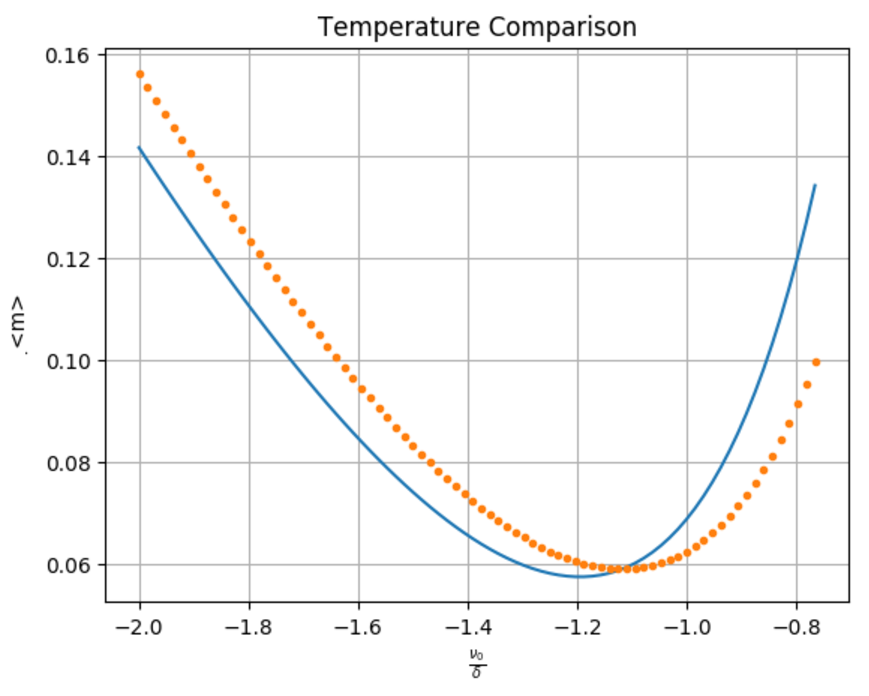
\includegraphics[scale=.55]{GraficaTemp.pdf} 
\caption{\textit{Comparación entre predicciones con y sin el término $\epsilon$} La línea puntuada representa la predicción sin dependencia temporal y la línea sólida representa la predicción con el término adicional. Esta resulta en un mínimo más pequeño de excitaciones posibles y en un corrimiento en el punto donde se espera encontrar este mínimo. Se utiliza $\kappa \ll \nu_0$}
\end{figure}

\chapter{Dependencia Temporal en la Frecuencia de la Cavidad}

Como se puede observar en el capítulo anterior, el cambio en el comportamiento predicho por el modelo con dependencia temporal es notorio. Sin embargo, durante todas las derivaciones se asume que la cavidad tiene un solo modo de frecuencia constante $\omega_c$. La frecuencia de resonancia de una cavidad de Fabry-Perot, asumiendo que su interior se encuentre en el vacío, está dada por

\begin{equation}
\omega_c = \frac{mc}{2L},
\end{equation} donde $c$ es la velocidad de la luz en el vacío, $m$ es algún entero y $L$ es la longitud de la cavidad. Al emplear un montaje optomecánico como el que se lleva a los resultados del capítulo anterior, $L$ deja de ser constante. Si el oscilador mecánico tiene oscilaciones de amplitud $A$ y se toma a $L_0$ como la longitud promedio de la cavidad, la longitud de la cavidad como función del tiempo viene dada por

\begin{equation}
L(t) = L_0 + A\nu(t)t
\end{equation} lo cual lleva a la frecuencia 

\begin{align}
\omega_c(t) =& \frac{mc}{2(L + A\nu(t)t)},\\
=& \frac{mc}{2L + 2A(\nu_0 + \epsilon cos(2\omega t))t)}
\end{align}



\bibliographystyle{unsrt}
\bibliography{Bib}

\end{document}